\documentclass[11pt, oneside]{article} 
\usepackage{geometry}
\geometry{letterpaper} 
\usepackage{graphicx}
	
\usepackage{amssymb}
\usepackage{amsmath}
\usepackage{parskip}
\usepackage{color}
\usepackage{hyperref}

\graphicspath{{/Users/telliott_admin/Dropbox/Tex/png/}}
% \begin{center} 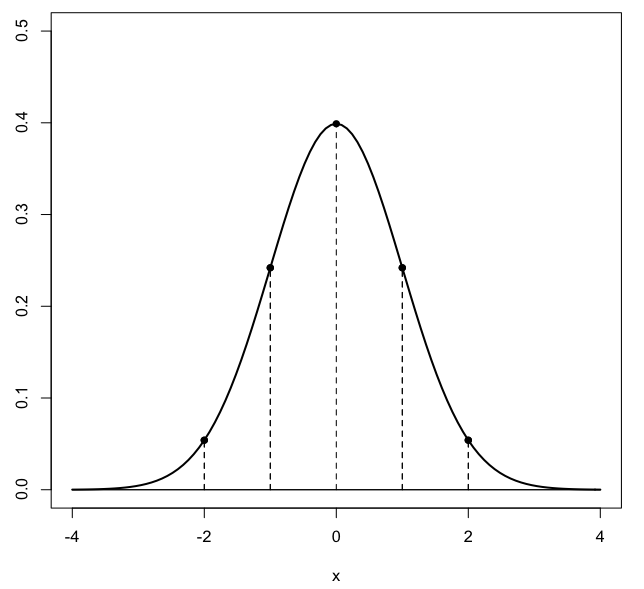
\includegraphics [scale=0.4] {gauss3.png} \end{center}

\title{Harmonic oscillator}
\date{}

\begin{document}
\maketitle
\Large

\label{sec:Harmonic_oscillator}

Here we look at the classical equations for oscillation, using as one of the sources the Physics lectures by Prof. Shankar.  The simplest example is called the mass and spring system.
\begin{center} 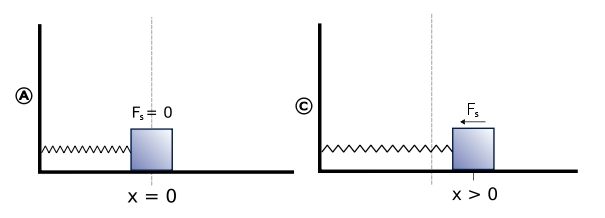
\includegraphics [scale=0.5] {spring1.png} \end{center}

In the picture, the left panel is the equilibrium position, while the right view is the mass displaced to the right by some distance $x$.  We pulled it there and have just released it.  The force due to the spring is $F = -kx$.  Not shown is the picture when the mass goes to the left of the equilibrium position and compresses the spring.  To begin with, we will use a frictionless table.  Without friction, the mass will oscillate back and forth forever.

We don't need vectors for this since we are working in one dimension.  By experiment, we find that the force is proportional to the displacement and directed toward the equilibrium position.  
\[ F = - kx \]
Newton's Law says that $F=ma$ so
\[ F = ma = m \ddot{x} = - kx \]
\[ \ddot{x} + \frac{k}{m} x = 0 \]
This equation is easy to solve.  We need something whose second derivative is minus itself, within some constant.  A good choice is
\[ x(t) = A \cos \omega t \]
We choose $\cos t$ rather than $\sin t$ because we want $x(0) \ne 0$.
\[ \ddot{x}(t) = - \omega^2 A \cos \omega t \]
so that
\[ \ [ \ - \omega^2 + \frac{k}{m} \ ] \ A \cos \omega t = 0 \]
$A$ corresponds to $x(0)$, which we want to be non-zero.  This equation is zero (for all $t$) only when 
\[ \frac{k}{m} = \omega^2 \]
\[ \omega = \sqrt{k/m} \]
Observe that $A$ can be anything we want.  It corresponds to the maximum amplitude of the oscillation, determined by how far we pull out the mass to start things off.

In contrast, $\omega$ is determined by the characteristics of the spring, and is inversely proportional to the mass.  $\omega$ is also related to the frequency of oscillation.  If $T$ is the time period for one complete oscillation, then $\omega T = 2 \pi$, or if $f$ is the frequency of oscillation, then $\omega = 2 \pi f$.

\subsection*{phase}

Finally, this solution assumes that $v_0 = 0$
\[ \dot{x}(t) = - \omega A \sin \omega t \]
\[ \dot{x}(0) = - \omega A \sin \omega (0) = 0 \]
That is more restrictive than necessary.  We can deal with this in various ways, one is to add a term containing the sine to $x(t)$
\[ x(t) =  A \cos \omega t + B \sin \omega t\]
\[ \dot{x}(t) =  - \omega A \sin \omega t + B \cos \omega t\]
\[ \dot{x}(0) = B = v_0 \]
Another way is to add a phase term to the angle, which doesn't change the derivatives
\[ x(t) =  A \cos \omega t + \phi \]
\[ \dot{x}(t) = - \omega A \sin \omega t + \phi \]
\[ \dot{x}(0) = v_0 = - \omega A \sin \phi \]

It is interesting to see why these amount to the same thing.  Recall
\[ \cos \omega t + \phi = \cos \omega t \cos \phi - \sin \omega t \sin \phi \]
But $\phi$ is a constant so if $-B = \sin \phi$ and $A = \cos \phi$
\[ \cos \omega t + \phi = A \cos \omega t + B \sin \omega t \]

However, for now we will agree to set our clock to zero when the mass has just been released and has zero velocity, at the maximum amplitude of the oscillation.

\subsection*{Conservation of Energy}
At this point, Prof. Shankar does this calculation
\[ x(t) = A \cos \omega t \]
\[ v = \dot{x} = - \omega A \sin \omega t \]
\[ E = \frac{1}{2}mv^2 + \frac{1}{2} kx^2 \]
\[ = \frac{1}{2}m \omega^2 A^2 \sin^2 \omega t + \frac{1}{2} k A^2 \cos^2 \omega t \]
But $\omega^2 = k/m$ so
\[ = \frac{1}{2}k A^2 \sin^2 \omega t + \frac{1}{2} k A^2 \cos^2 \omega t \]
\[ E = \frac{1}{2}k A^2 \]
Not only is this independent of time, but we can write
\[ \frac{1}{2}k A^2 = \frac{1}{2}mv^2 + \frac{1}{2} kx^2 \]
Given $A$ and $x$, we can find $v$, and so on.

\end{document}  